\documentclass[a4paper,12pt,french]{article}

\usepackage[cours]{../../Style}

%\usepackage[theorems]{tcolorbox}

%\newtcbtheorem
%{defi}{Définition}
%{colback=red!5,colframe=red!60!black!80,fonttitle=
%\sffamily\bfseries}{th}

% Début du document
%%%%%%%%%%%%%%%%%%%
\begin{document}

\title{Fonctions polynomiales de degré 2}
\maketitle

\begin{programme}
\item représentations graphiques des fonctions : $x \mapsto ax^2,x \mapsto ax^2+b, x \mapsto a(x-x_1)(x-x_2)$
\item axes de symétrie ;
\item racines et signe d'un polynôme de degré 2 donné sous forme factorisée (le calcul des
racines à l'aide du discriminant ne figure pas au programme).
\item Compétences
\begin{itemize}
\item Associer une parabole à une expression algébrique de degré 2
\item Déterminer des éléments caractéristiques de la fonction $x \mapsto a(x-x_1)(x-x_2)$: Signe, extremum, allure, axes de symétrie
\item Vérifier qu'une valeur conjecturée est racine d'un polynôme de degré 2
\item Savoir factoriser dans des cas simples une expression du second degré connaissant une racine.
\item Utiliser la forme factorisée d'un poly pour trouver ses racines et étudier son signe.
\end{itemize}
\item déterminer le signe d'une expression factorisée du second degré
\item résoudre une équation ou une inéquation du premier degré, une équation du type $x^2=a$ avec $a \geq 0$.
\end{programme}

\section{Généralités}

\begin{defin}
On appelle fonction polynomiale de degré $2$ toute fonction $$\fonction f {\R} {\R} x {ax^2+bx+c}$$ Où $a,\ b,\ c \in \R$ et \textbf{$a \neq 0$}.
\end{defin}

\begin{exs}
$f:x \mapsto x^2 \ , \ g:x \mapsto 3x^2-4$ et $h:x \mapsto 2-0,3x^2$ sont des fonctions polynomiales de degré 2.
\end{exs}

\rem[eleve]{L'appellation est un peu lourde... On dira plutôt fonction de degré 2.}

\rem{Exo 1f\\Graphe d'une fonction au choix}

\begin{prop}
La représentation graphique d'une fonction de degré 2 est une parabole.
\end{prop}

\begin{exs}
\begin{centrer}
\begin{tikzpicture}
\begin{axis}[
styleglobal,
hauteurproptick,
width=0.7*\linewidth,
xmin=-7, xmax=7,
ymin=-4.5, ymax=6,
xtick distance=1,
ytick distance=1,
domain=(-7:7),
]
\addplot[styleplot]{x^2} node[pos=0.55,right] {$\mathscr C_f:\fbox{a>0}$};
\addplot[styleplot,color=red,domain=(-6:-2)]{3*(x+4)^2-4} node[pos=0.82,left] {$\mathscr C_g:\fbox{a>0}$};
\addplot[color=blue,styleplot]{2-0.25*(x-1)^2} node[pos=0.8,right] {$\mathscr C_h:\fbox{a<0}$};
\end{axis}
\end{tikzpicture}
\end{centrer}
\end{exs}

\rem{Montrer sur geogebra l'effet obtenu en changeant $a$ et $c$}

\begin{rmq}
Le terme constant (sans $x$, c'est-à-dire $c$) est l'ordonnée à l'origine de la parabole. Changer $c$ décale la parabole vers le haut ou vers le bas.
\end{rmq}

\begin{proprs}
Soit $f$ une fonction de degré 2.
\begin{itemize}
\item Si $a \geq 0$,  $f$ est décroissante puis croissante: elle branche vers le haut.
\item Si $a \leq 0$,  $f$ est croissante puis décroissante: elle branche vers le bas.
\end{itemize}
\end{proprs}

\begin{defin}
On appelle sommet d'une parabole le point où elle change de direction. C'est le point le plus bas si $a > 0$, le point le plus haut sinon.

\begin{centrer}
\begin{tikzpicture}
\begin{axis}[
styleglobal,
hauteurproptick,
width=0.7*\linewidth,
xmin=-3, xmax=5,
ymin=-1.5, ymax=1.5,
xtick distance=1,
ytick distance=1,
domain=(-6:6),
]
\addplot[styleplot]{0.7-0.5*(x-1.3)^2} node[pos=0.53,right] {$\mathscr C_f$};
\node[stylepoint,fill=red] (S) at (1.3,0.7) {};
\node (sommet) at (2.3,1.2) {Sommet};
\draw[->,>=latex,thick] (sommet.west) to[bend right=10] (S);
\draw[color=DarkRed,thick,densely dashed] (S) -- (1.3,0) node[pos=1,below] {$s$};
\draw[color=DarkRed,thick,densely dashed] (S) -- (0,0.7) node[pos=1,left] {$f(s)$};
\end{axis}
\end{tikzpicture}
\end{centrer}

\end{defin}

\begin{proprs}
On se donne $f$ une fonction de degré 2 et $s$ l'abscisse du sommet de la parabole associée.
\begin{itemize}
\item Les coordonnées de son sommet sont donc $(s,f(s))$.
\item La parabole associée possède pour axe de symétrie la droite parallèle a l'axe des ordonnées (verticale) passant par son sommet.
\item On en déduit le tableau de variations de $f$:

\compo
{
\begin{center}
Si $a>0$:
\begin{tikzpicture}
\tkzTabInit[lgt=1.2,espcl=2.5]{$x$ /1, $f(x)$/2}{$- \infty$, $s$, $+ \infty$}
\tkzTabVar{+/$+ \infty$, -/ $f(s)$, +/ $+\infty$}
\end{tikzpicture}
\end{center}
}
{
\begin{center}
Si $a<0$:
\begin{tikzpicture}
\tkzTabInit[lgt=1.2,espcl=2.5]{$x$ /1, $f(x)$/2}{$- \infty$, $s$, $+ \infty$}
\tkzTabVar{-/$- \infty$, +/ $f(s)$, -/ $-\infty$}
\end{tikzpicture}
\end{center}
}
\end{itemize}
\end{proprs}

\rem[eleve]{On verra dans la suite comment trouver algébriquement (par le calcul) les coordonnées de ce sommet, dans des cas particuliers.}

\rem{Exo 2f}

\section{Fonctions $x \mapsto ax^2+c$}

\rem{Faire tracer la représentation graphique d'une fonction de degré 2 à chacun ( calculatrice ou non ). En déterminer les coordonnées du sommet. Remarques?}

\begin{proprs}
Soit $f:x \mapsto ax^2+c$ une fonction de degré 2.
\begin{itemize}
\item Les paraboles d'équation $y=ax^2+c$ ont pour axe de symétrie l'axe des ordonnées.
\item Les coordonnées du sommet de cette parabole sont $(0;c)$.
\end{itemize}
\end{proprs}

\begin{exs}
\begin{centrer}
\begin{tikzpicture}
\begin{axis}[
styleglobal,
%hauteurproptick,
width=0.7*\linewidth,
xmin=-7, xmax=7,
ymin=-4, ymax=5,
xtick distance=1,
ytick distance=2,
y post scale=0.5,
domain=(-7:7),
]
\addplot[styleplot]{x^2} node[pos=0.55,right] {$\mathscr C_f:\fbox{a>0}$};
\addplot[styleplot,color=red,domain=(-2:2)]{3*(x)^2-3} node[pos=0.54,right] {$\mathscr C_g:\fbox{a>0}$};
\addplot[color=blue,styleplot]{2-0.25*(x)^2} node[pos=0.7,right] {$\mathscr C_h:\fbox{a<0}$};
\end{axis}
\end{tikzpicture}
\end{centrer}
\end{exs}

\begin{ex}
Soit $f:x \mapsto 5x^2-2$. Les coordonnées du sommet de la parabole associée sont $(0;-2)$.
\end{ex}

\begin{rems}
Sommet, symétries: Exos 20,21,23,22,(24) p120\\
Variations: Exo 49 p122\\
Représentation, variations: Exo 46 p122\\
Equations: Exos 52,53,54 p123
\end{rems}

\begin{methode}
Pour déterminer l'expression d'une fonction $f:x \mapsto ax^2+c$ à partir de sa représentation graphique, on lit d'abord $c$ en regardant l'ordonnée à l'origine, puis on détermine $a$ en résolvant une équation.
\end{methode}

\begin{ex}
\compo[0.7]
{
On a représenté une fonction $f:x \mapsto ax^2+c$ sur le repère ci-contre.

\

On voit directement que $c=1$, d'où $f:x \mapsto ax^2+1$.

\

On se donne maintenant un point sur la courbe de $f$, par exemple $A(1;3)$. Cela signifie que $f(1)=3$, autrement dit $a \times 1^2 + 1=3$, soit donc $a+1=3$, d'où $a=2$.

\

On a alors $f:x \mapsto 2x^2+1$.
}
{
\vspace{-9mm}
\begin{centrer}
\begin{tikzpicture}
\begin{axis}[
styleglobal,
hauteurproptick,
width=0.9*\linewidth,
xmin=-2.5, xmax=2.5,
ymin=-0.5, ymax=5,
xtick distance=1,
ytick distance=1,
domain=(-6:6),
]
\addplot[styleplot]{2*x^2+1} node[pos=0.525,right] {$\mathscr C_f$};
\node[stylepoint,fill=blue,label={-60:A}] at (1,3) {};
\end{axis}
\end{tikzpicture}
\end{centrer}
}
\end{ex}

\rem{Exo 3f\\Exo 22p121(méthode 2)\\Préciser: Dans le livre on voit $ax^2+b$, à voir ...}

\section{Fonctions $x \mapsto a(x-x_1)(x-x_2)$}
\subsection{Généralités}

\begin{prop}
Les fonctions du type $f:x \mapsto a(x-x_1)(x-x_2)$ sont des fonctions de degré 2. On dit que cette forme est l'écriture factorisée de $f$ (lorsqu'elle existe).
\end{prop}

\begin{fait}
En effet, $\begin{aligned}[t]a(x-x_1)(x-x_2) & =a(x^2-xx_2-xx_1+x_1x_2) \\ & =ax^2-axx_2-axx_1+ax_1x_2 \\ & =ax^2-(ax_1+ax_2)x+ax_1x_2 \end{aligned}$

Donc $a(x-x_1)(x-x_2) =a x^2+b x + c$ avec $b = -(ax_1+ax_2)$ et $c=ax_1x_2$.
\end{fait}

\begin{rems}
Exos 79,80,(81->83) p125\\
Remarque par rapport à la suite?
\end{rems}

\begin{defin}
Soit $f$ une fonction de degré 2. On appelle \textbf{racines} de $f$ les solutions de l'équation $f(x)=0$. Ce sont donc les abscisses des points d'intersection entre la courbe représentative de $f$ et l'axe des abscisses.
\begin{centrer}
\begin{tikzpicture}
\begin{axis}[
styleglobal,
hauteurproptick,
width=0.7*\linewidth,
xmin=-2, xmax=6,
ymin=-1, ymax=2,
xtick distance=1,
ytick distance=1,
domain=(-6:6),
]
\addplot[styleplot]{0.5*(x-1)*(x-3)} node[pos=0.52,right] {$\mathscr C_f$};
\node[stylepoint,fill=red] (S) at (2,-0.5) {};
\node (sommet) at (3,-0.7) {Sommet};
\draw[->,>=latex,thick] (sommet.west) to[bend left=10] (S);
\node[stylepoint,fill=blue] (x1) at (1,0) {};
\node[stylepoint,fill=blue] (x2) at (3,0) {};
\node (racines) at (2,1) {Racines};
\draw[->,>=latex,thick] (racines) to[bend right=10] (x1);
\draw[->,>=latex,thick] (racines) to[bend left=10] (x2);
\end{axis}
\end{tikzpicture}
\end{centrer}
\end{defin}

\begin{rmq}
Si $f(x)=a(x-x_1)(x-x_2)$ $(a \neq 0)$, les racines de $f$ sont $x_1$ et $x_2$.
\end{rmq}

\begin{fait}
En effet, $\begin{aligned}[t] a(x-x_1)(x-x_2)=0 & \Leftrightarrow a=0 \text{ ou } x-x_1=0 \text{ ou } x-x_2=0 \\ & \Leftrightarrow x=x_1 \text{ ou } x=x_2 \end{aligned}$
\end{fait}

\begin{ex}
Les racines de la fonction $f:x \mapsto -2(x-2)(x+4)$ sont 2 et $-4$.
\begin{centrer}
\begin{tikzpicture}
\begin{axis}[
styleglobal,
%hauteurproptick,
width=0.7*\linewidth,
xmin=-6, xmax=4,
ymin=-5, ymax=20,
xtick distance=1,
ytick distance=5,
domain=(-6:6),
y post scale=0.2,
]
\addplot[styleplot]{-2*(x-2)*(x+4)} node[pos=0.52,right] {$\mathscr C_f$};
\node[stylepoint,fill=blue] (x1) at (2,0) {};
\node[stylepoint,fill=blue] (x2) at (-4,0) {};
\end{axis}
\end{tikzpicture}
\end{centrer}
On voit alors que la parabole associée par $f$ coupe l'axe des abscisses en $M(2;0)$ et $N(0;-4)$.
\end{ex}

\rem{Exos 84,85 p125}

\begin{propr}
Soit $f:x \mapsto a(x-x_1)(x-x_2)$ avec $a \neq 0$. On pose $s=\frac{x_1+x_2} 2$. Alors le sommet de la parabole associée a pour coordonnées $(s,f(s))$.
\end{propr}

\begin{ex}
Pour la parabole précédente, on a $s=\frac{2-4} 2=-1$, et:
$$\begin{aligned}[t]
f(s)&=f(-1)\\
&=-2(-1-2)(-1+4)\\
&=-2 \times (-3) \times 3\\
&=18
\end{aligned}
$$
Les coordonnées du sommet de la parabole sont donc $(-1;18)$.
\end{ex}

\rem{Exos 26,27,29 p121}

\subsection{Factorisation}

\begin{fait}
Soit $f:x \mapsto ax^2+b+c$. Ceci est l'écriture développée de $f$. On souhaite retrouver l'écriture factorisée $f(x)=a(x-x_1)(x-x_2)$.
\end{fait}

\begin{rmq}
Le $a$ qui apparait dans la forme développée et factorisée est le même.
\end{rmq}

\begin{methode}
Si l'on connait une racine $x_1$ de $f$, on peut retrouver l'écriture factorisée de $f$ par identification.
\end{methode}

\begin{ex}
Soit $f:x \mapsto 3x^2-9x+6$. On nous dit que $1$ est une racine de $f$. De plus, on a $a=3$.

On sait alors qu'on peut écrire $f(x)=3(x-1)(x-x_2)$ avec $x_2 \in \R$.

\vspace{1mm}

\textbf{Première méthode:}  Développons cette expression:
$$\begin{aligned}[t]
f(x)&=3\left( x^2-x \times x_2-x+x_2 \right)\\
&=3x^2-3 \times x_2 \times x -3x+3x_2\\
&= 3x^2+{\color{DarkRed}(-3-3x_2)}x+{\color{DarkBlue}3x_2}\\
\text{On a de plus } f(x)&=3x^2 {\color{DarkRed}-9}x+{\color{DarkBlue}6}
\end{aligned}$$

Le {\color{DarkBlue} dernier coefficient} nous donne donc $3x_2=6$ soit alors $x_2=2$.

On en déduit que $f(x)=3(x-1)(x-2)$.

\vspace{1mm}

\textbf{Seconde méthode:} On calcule $f(0)$ de deux manières différentes:

$$\hfill \begin{aligned}[t]
f(0)&=3 \times 0^2 - 9 \times 0 +6\\
&=6\\
\end{aligned}
\ \hspace{2cm} \
\begin{aligned}[t]
f(0)&=3(0-1)(0-x_2)\\
&=3 \times (-1) \times (-x_2)\\
&=-3 \times (-x_2)\\
&=3x_2 \\
\end{aligned} \hfill \ $$

On retrouve alors l'équation précédente: $3x_2=6$ d'où $x_2=2$ puis $f(x)=3(x-1)(x-2)$.

\end{ex}

\begin{rems}
Exo 28 p121 \\
Exos 60 -> 66 p123
\end{rems}

\subsection{Etude du signe}

\begin{methode}
Pour dresser algébriquement le tableau de signes d'une fonction du type $f:x \mapsto a(x-x_1)(x-x_2)$, on peut étudier le signe des deux fonctions affines qui la composent et d'utiliser la règle des signes.
\end{methode}

\begin{ex}
Soit $f:x \mapsto 0,5(x-1)(x+3)$. Cette fonction est donc composée des deux fonctions affines $x \mapsto x-1$ et $x \mapsto x+3$. On peut d'abord dresser le tableau de signes de ces deux fonctions:

\compo[0.5]
{
\begin{center}
\begin{tikzpicture}
\tkzTabInit[lgt=1.2,espcl=2]{$x$ /1, $x-1$/1}{$- \infty$, $1$, $+ \infty$}
\tkzTabLine{,-,z,+,}
\end{tikzpicture}
\end{center}
}
{
\begin{center}
\begin{tikzpicture}
\tkzTabInit[lgt=1.2,espcl=2]{$x$ /1, $x+3$/1}{$- \infty$, $-3$, $+ \infty$}
\tkzTabLine{,-,z,+,}
\end{tikzpicture}
\end{center}
}

\

On peut alors combiner ces tableaux pour dresser le tableau de signes de $f$:

\begin{centrer}
\begin{tikzpicture}
\tkzTabInit[lgt=3]{$x$ /1, $x-1$/1, $x+3$/1,$(x-1)(x+3)$/1,$f(x)$/1}{$- \infty$, $-3$, $1$, $+ \infty$}
\tkzTabLine{,-,t,-,z,+}
\tkzTabLine{,-,z,+,t,+}
\tkzTabLine{,+,z,-,z,+}
\tkzTabLine{,+,z,-,z,+}
\end{tikzpicture}
\end{centrer}

On peut donc lire sur ce tableau que l'ensemble des solutions de l'inéquation $f(x) \geq 0$ est: $$S=]-\infty ;-3] \cup [1;+\infty [$$

On peut vérifier que l'on obtient le même tableau par lecture graphique.

\begin{centrer}
\begin{tikzpicture}
\begin{axis}[
styleglobal,
width=0.6*\linewidth,
xmin=-8, xmax=6,
ymin=-3, ymax=5,
domain=(-6:6),
]
\addplot[styleplot]{0.5*(x-1)*(x+3)} node[pos=0.52,right] {$\mathscr C_f$};
\node at (0,1) {};
\end{axis}
\end{tikzpicture}
\end{centrer}
\end{ex}

\begin{rems}
Exos 72 -> 74 p124\\
Exos 88 (-> 90) p125
\end{rems}

\begin{deroule}
\item \textbf{Total: 3.5 semaines}
\item Semaine 1
\begin{itemize} 
\item 30m - Cours I partie 1: Définitions et exo
\item 15m - Graphe de $x \mapsto x^2$
\item 1h - Cours: Représentation graphique, sommet, variations, exo
\item 30m - Cours II: Généralités+Exos
\end{itemize}
\item Semaine 2
\begin{itemize}
\item 1h - Suite
\item 1h - II.2 + Exos
\item 45m - III.1.1 + Exos
\item 45m - III.1.2 + Exos
\end{itemize}
\item Semaine 3
\begin{itemize}
\item 30m - Suite
\item 45m: III.1.3 + Exos
\item 1h: III.2 + Exos
\item 1h: III.3 + Exos
\end{itemize}
\end{deroule}

\end{document}
